% Velicina i tip stranice
\documentclass[a4paper]{article}

%% Dodatak za margine
\usepackage[a4paper,top=2cm,bottom=2cm,left=2cm,right=2cm,marginparwidth=1.75cm]{geometry}

%% Dodaci za jezik
\usepackage{hyphsubst}
\usepackage{ucs}
\usepackage[T1]{fontenc}
\usepackage[utf8x]{inputenc}
\usepackage[serbian]{babel}

%% Korisni dodaci
\usepackage{amsfonts}
\usepackage{amsmath}
\usepackage{amssymb}
\usepackage{booktabs}
\usepackage{enumerate}
\usepackage{enumitem}
\usepackage{esint}
\usepackage{gensymb}
\usepackage{graphicx}
\usepackage[hidelinks]{hyperref}
\usepackage{listings}
\usepackage{lipsum}
\usepackage{setspace}
\usepackage{lmodern}
\usepackage{mathrsfs}
\usepackage{mathtools}
\usepackage{minted}
\usepackage{multicol}
\usepackage{multicol}
\usepackage{csquotes}
\usepackage{physics}

% Označavanje figura
\usepackage{caption}
\captionsetup{justification=justified,
   format=plain,font=small,labelfont=sc,margin=50pt}

% Formatiranje
\setstretch{1.2}
\setlength{\parskip}{1em}
\setlength{\parindent}{0em}
\setlength{\abovedisplayskip}{0pt}
\setlength{\belowdisplayskip}{0pt}

% Uputstvo:
% U svoj TeX dokument na vrh dodajte
% % Velicina i tip stranice
\documentclass[a4paper]{article}

%% Dodatak za margine
\usepackage[a4paper,top=2cm,bottom=2cm,left=2cm,right=2cm,marginparwidth=1.75cm]{geometry}

%% Dodaci za jezik
\usepackage{hyphsubst}
\usepackage{ucs}
\usepackage[T1]{fontenc}
\usepackage[utf8x]{inputenc}
\usepackage[serbian]{babel}

%% Korisni dodaci
\usepackage{amsfonts}
\usepackage{amsmath}
\usepackage{amssymb}
\usepackage{booktabs}
\usepackage{enumerate}
\usepackage{enumitem}
\usepackage{esint}
\usepackage{gensymb}
\usepackage{graphicx}
\usepackage[hidelinks]{hyperref}
\usepackage{listings}
\usepackage{lipsum}
\usepackage{setspace}
\usepackage{lmodern}
\usepackage{mathrsfs}
\usepackage{mathtools}
\usepackage{minted}
\usepackage{multicol}
\usepackage{multicol}
\usepackage{csquotes}
\usepackage{physics}

% Označavanje figura
\usepackage{caption}
\captionsetup{justification=justified,
   format=plain,font=small,labelfont=sc,margin=50pt}

% Formatiranje
\setstretch{1.2}
\setlength{\parskip}{1em}
\setlength{\parindent}{0em}
\setlength{\abovedisplayskip}{0pt}
\setlength{\belowdisplayskip}{0pt}

% Uputstvo:
% U svoj TeX dokument na vrh dodajte
% % Velicina i tip stranice
\documentclass[a4paper]{article}

%% Dodatak za margine
\usepackage[a4paper,top=2cm,bottom=2cm,left=2cm,right=2cm,marginparwidth=1.75cm]{geometry}

%% Dodaci za jezik
\usepackage{hyphsubst}
\usepackage{ucs}
\usepackage[T1]{fontenc}
\usepackage[utf8x]{inputenc}
\usepackage[serbian]{babel}

%% Korisni dodaci
\usepackage{amsfonts}
\usepackage{amsmath}
\usepackage{amssymb}
\usepackage{booktabs}
\usepackage{enumerate}
\usepackage{enumitem}
\usepackage{esint}
\usepackage{gensymb}
\usepackage{graphicx}
\usepackage[hidelinks]{hyperref}
\usepackage{listings}
\usepackage{lipsum}
\usepackage{setspace}
\usepackage{lmodern}
\usepackage{mathrsfs}
\usepackage{mathtools}
\usepackage{minted}
\usepackage{multicol}
\usepackage{multicol}
\usepackage{csquotes}
\usepackage{physics}

% Označavanje figura
\usepackage{caption}
\captionsetup{justification=justified,
   format=plain,font=small,labelfont=sc,margin=50pt}

% Formatiranje
\setstretch{1.2}
\setlength{\parskip}{1em}
\setlength{\parindent}{0em}
\setlength{\abovedisplayskip}{0pt}
\setlength{\belowdisplayskip}{0pt}

% Uputstvo:
% U svoj TeX dokument na vrh dodajte
% \input{./dataset/izvestaj.tex}
% kako biste preuzeli podešavanja za izveštaj,
% slično fajlu smernice.tex

% kako biste preuzeli podešavanja za izveštaj,
% slično fajlu smernice.tex

% kako biste preuzeli podešavanja za izveštaj,
% slično fajlu smernice.tex


\title{Određivanje ubrzanja zemljine teže matematičkim klatnom}
\author{Petar Petrović}

\begin{document}

\maketitle

\section{Uvod}

Matematičko klatno predstavlja telo zanemarljivih dimenzija i značajne mase okačeno o neistegljivu nit zanemarljive mase a značajne dužine. Ovakvo klatno je realno klatno koje je najbliže idealizovanom klatnu za koje važe neki jednostavni zakoni (idealizovano klatno se predstavlja kao materijalna tačka okačena o neistegljivu nit bez mase).
\par
Kretanje matematičkog klatna se vrši po krugu poluprečnika $l$, gde je $l$ dužina klatna (Slika \ref{im:idealnoklatno}). Prema tome, ovakvo kretanje u opštem slučaju ne predstavlja prosto harmonijsko kretanje.

\begin{center}
    \label{im:idealnoklatno}
    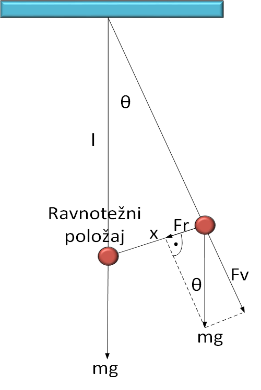
\includegraphics[height=8cm,keepaspectratio]{klatno.png}
    \captionof{figure}{Matematičko klatno}
\end{center}

Samo klatno se kreće pod uticajem gravitacione sile $mg$, međutim, na samo kretanje direktno utiče samo komponenta $F = mg \sin \theta$, dok druga komponenta vrši zatezanje niti.
\par
Za male uglove $\theta$ (kada važi aproksimacija $\sin \theta \approx \theta$), imamo da je pređeni put od ravnotežne tačke:

\begin{equation}
    \label{eq:aproksimacija}
    l\theta \approx l \sin \theta = l \frac{x}{l} = x
\end{equation}

Odavde vidimo da je pređeni put približno jednak rastojanju x od vertikalne ose. Dalje, kada iskoristimo da je $\sin\theta = \frac{x}{l}$, imamo da je: $F = mg \tfrac{x}{l}$ odnosno, $F = kx$ za $k = \tfrac{mg}{l}$.

Na osnovu ovoga, i (\ref{eq:aproksimacija}), možemo posmatrati kretanje matematičkog klatna kao prosto harmonijsko kretanje, za koje znamo da važi

\begin{equation}
    T = 2 \pi \sqrt{\frac{m}{k}}
\end{equation}

gde je $T$ period oscilacija. Na osnovu ovoga, za dobijeno $k$, imamo da je

\begin{equation}
    \label{eq:period}
    T = 2 \pi \sqrt{\frac{l}{g}}
\end{equation}

Jasno je da se matematičko klatno može iskoristiti za određivanje ubrzanja zemljine teže pomoću obrasca (\ref{eq:period}) (ali samo za dovoljno male amplitude oscilovanja).

\section{Aparatura}

Oprema se sastoji od jednog stalka na kome je montirano matematičko klatno. Sama dužina klatna se može jednostavno izmeniti namotavanjem i odmotavanjem kotura $K$. Samo telo $m$ je okačeno pomoću neistegljive niti za kotur $K$.

Na vertikalnom stubu stalka se nalazi i skala kojom se može odrediti dužina klatna. Ona je tako podešena da pokazuje rastojanje upravo od tačke na kojoj je zakačena nit (tačka ispod kotura odakle nit ide vertikalno).

\section{Metod rada}

Pomoću (\ref{eq:period}), jednostavnim transformacijama, dolazimo do zaključka da postoji linearna zavisnost kvadrata perioda $T^2$ i dužine klatna $l$

\begin{equation}
    \label{eq:kvadratperioda}
    T^2 = \frac{4 \pi^2}{g} l
\end{equation}

Promenama dužine klatna, i merenjem perioda oscilovanja za svaku dužinu ćemo dobiti rezultate koji će nam omogućiti da odredimo koeficijent pravca prave (\ref{eq:kvadratperioda}), tj.
$T^2 = a \cdot l$, za $a = \frac{4 \pi^2}{g}$.

Prema tome, iz određenog koeficijenta pravca $a$ linearne zavisnosti, lako ćemo odrediti ubrzanje zemljine teže g kao

\begin{equation}
    \label{eq:gravitacija}
    g = \frac{4 \pi^2}{a}
\end{equation}

Pri merenju dužine klatna, merićemo dužinu sa i bez kuglice (odnosno tela na kraju niti), i zatim uzimati aritmetičku sredinu ove dve dužine kao dužinu klatna. Ovo radimo pod pretpostavkom da je telo homogeno i simetrično. Zatim je potrebno izmeriti period oscilovanja za svaku dužinu klatna (a ovo radimo sa većim brojem oscilacija kako bi smanjili grešku).

Sama dužina klatna je aritmetička sredina vrednosti za dužinu $l_1$ klatna bez tela $m$, i dužinu $l_2$ klatna sa telom $m$. Pri čitanju vrednosti za $l_1$ i $l_2$ potrebno je da pogled bude normalan na skalu i u visini vrednosti koja se čita. Telo treba izvesti iz ravnotežnog položaja kako bi počelo da osciluje, i tada hronometrom meriti vreme oscilacija. Potrebno je da se oscilacije vrše u jednoj ravni.

\section{Rezultati}

Za svaku pojedinačnu dužinu klatna l se meri tri puta period $50$ oscilacija. Zatim se kao stvarni period $50$ oscilacija uzima aritmetička sredina dobijenih vrednosti. Zatim, deljenjem te vrednosti sa brojem oscilacija $N = 50$ se dobija osnovni period oscilovanja matematičkog klatna dužine $l$.

\begin{table}[h!]
    \centering
    \begin{tabular}{|c|c|c|c|c|c|c|c|c|c|c|}
      \hline
         & $l_1$ [cm] & $l_2$ [cm] & $l$ [cm] & $N$ & $t$ [s] & $\Delta t$ [s] & $T$ [s] & $\Delta T$ [s] & $T$ [s] & $\Delta T$ [s] \\ \hline
      1. & 9.4        & 10.7       & 10.05    & 50 & 32.4     & 0.1            & 0.65    & 0.002 & 0.420  & 0.003 \\ \hline
      2. & 19.5       & 20.8       & 20.15    & 50 & 45.1     & 0.13           & 0.90    & 0.003 & 0.815  & 0.006 \\ \hline
      3. & 26.0       & 27.3       & 26.65    & 50 & 54.1     & 0.13           & 1.08    & 0.003 & 1.173  & 0.007 \\ \hline
      4. & 40.1       & 41.4       & 40.75    & 50 & 64.5     & 0.13           & 1.29    & 0.003 & 1.662  & 0.008 \\ \hline
      5. & 49.9       & 51.2       & 50.55    & 50 & 71.5     & 0.13           & 1.43    & 0.003 & 1.054  & 0.008 \\ \hline
      6. & 59.7       & 61.0       & 60.35    & 50 & 77.3     & 0.13           & 1.54    & 0.003 & 1.390  & 0.008 \\ \hline
      7. & 70.3       & 71.6       & 70.95    & 50 & 84.7     & 0.13           & 1.69    & 0.003 & 1.870  & 0.010 \\ \hline
      8. & 80.7       & 81.9       & 81.30    & 50 & 90.7     & 0.13           & 1.81    & 0.003 & 1.290  & 0.020 \\ \hline
    \end{tabular}
    \label{tab:rezulatati}
    \caption{Zavisnost kvadrata perioda od dužine klatna}
\end{table}

Ucrtavanjem eksperimentalno dobijenih podataka na grafik $T^2 = a \cdot l$, i provlačenjem ove pravešto je moguće tačnije kroz date tačke, možemo uočiti dve konkretne vrednosti za $T^2$ za odabrane vrednosti $l$. Naime, za $l_1 = 0.0 cm$ vidimo da je ${T_1}^2 = 0,02s^2$, odnosno, za $l_2 = 80.0 cm$ je ${T_2}^2 = 3,25s^2$. Prema tome, imamo da je
\begin{equation}
    a = \frac{T_1^2 - T_2^2}{l_1 - l_2} = 0.0404 \tfrac{s^2}{cm}
\end{equation}
Relativnu grešku $\Delta a / a$ određujemo kao
\begin{equation}
    \frac{\Delta a}{a} = 2 \cdot \frac{T_1 \Delta T_1 + T_2 \Delta T_2}{T_1^2 - T_2^2} + \frac{\Delta l_1 + \Delta l_2}{l_1 - l_2} = 0.0142
\end{equation}

Odavde, i iz (\ref{eq:gravitacija}) imamo da je

\begin{equation}
    g = (9.77 \pm 0.013) \tfrac{m}{s^2}
\end{equation}

konačno:

\begin{equation}
    \boxed{
      g = (9.80 \pm 0.02) \tfrac{m}{s^2}
    }
\end{equation}

\section{Zaključak}

Iz priloženih rezultata prethodnih merenja može se zaključiti da se dobijena vrednost ubrzanja zemljine teže podudara sa teorijski utvrđenom vrednošću.

\end{document}
